
\documentclass{article}

%\usepackage{mslapa}
\usepackage{hyperref}
\usepackage{amsmath}
\usepackage{graphicx}
\usepackage{ulem}
\usepackage{vmargin}
\usepackage{tabularx}
\usepackage{sectsty}
\usepackage{pbox}
\usepackage{bigstrut}
\usepackage{enumerate}
\usepackage{listings}
\usepackage{parskip}   % space paragraphs but dont indent
\usepackage{verbatim}  % \verbatiminput{file}

\setpapersize{USletter}
%\sectionfont{\normalsize}
%\subsectionfont{\normalsize}
\setmarginsrb{1.0in}{1.0in}{1.0in}{1.0in}{0in}{0.25in}{0in}{0.20in}

% configure \bigstrut size
% This configures spacing above and below rows in a tabularx.
%\renewcommand{\bigstrutjot}{6pt}
\renewcommand{\bigstrutjot}{2.0\jot}

\providecommand{\e}[1]{\ensuremath{\times 10^{#1}}}

\raggedright

\begin{document}

% {{{ Cover Page

\null
\thispagestyle{empty}
\vspace{1in}
\centerline{\bf EECE 311}
\centerline{\bf Fall 2011}
\centerline{\bf}
\centerline{\bf Lab Report \#5}
\centerline{\bf Modeling and Analyzing RLC circuits with SPICE}
%\centerline{\bf Section 4}
%\centerline{\bf 9/13/2011} % date turned in
\centerline{\bf 10/11/2011}  % date lab performed

\vspace{0.5in}
% signature area
\begin{center}
\begin{tabularx}{\textwidth}[b]{X l l}
Signature & Printed Name & Date \\
\hline
\multicolumn{1}{|X|}{} & \multicolumn{1}{|l|}{\bigstrut \bf Jeremiah Mahler} & \multicolumn{1}{|l|}{\bf Oct 25, 2011} \\
\hline
%\multicolumn{1}{|X|}{} & \multicolumn{1}{|l|}{\bigstrut \bf Marvanee Johnson} & \multicolumn{1}{|l|}{\bf Sep 14, 2011} \\
%\hline
\end{tabularx}
\end{center}


\vfill
\pagebreak
% }}}

\tableofcontents

\pagebreak

% {{{ Objective
\section{Objective}

The objective of this laboratory exercise is to learn and gain
experience analyzing and simulating the behavior of first
order RC or RL circuits and second order RLC circuits under transient
conditions using a SPICE simulator.

% }}}

% {{{ Equipment
\section{Equipment}

To perform the circuit simulation the Ngspice\cite{NGSPICE} SPICE\cite{wiki:SPICE} simulator was used.
Other SPICE simulators such as Pspice\cite{wiki:Pspice} and Orcad\cite{ORCAD}
should work as well.

% }}}

% {{{ Procedure
\section{Procedure}

The circuit to be analyzed (Figure \ref{fig:circuit}) consists of
resistors, voltage sources, a capacitor, a inductor and a switch.
The switch alternates the capacitor between two parts of the circuit.

\begin{figure}
\center
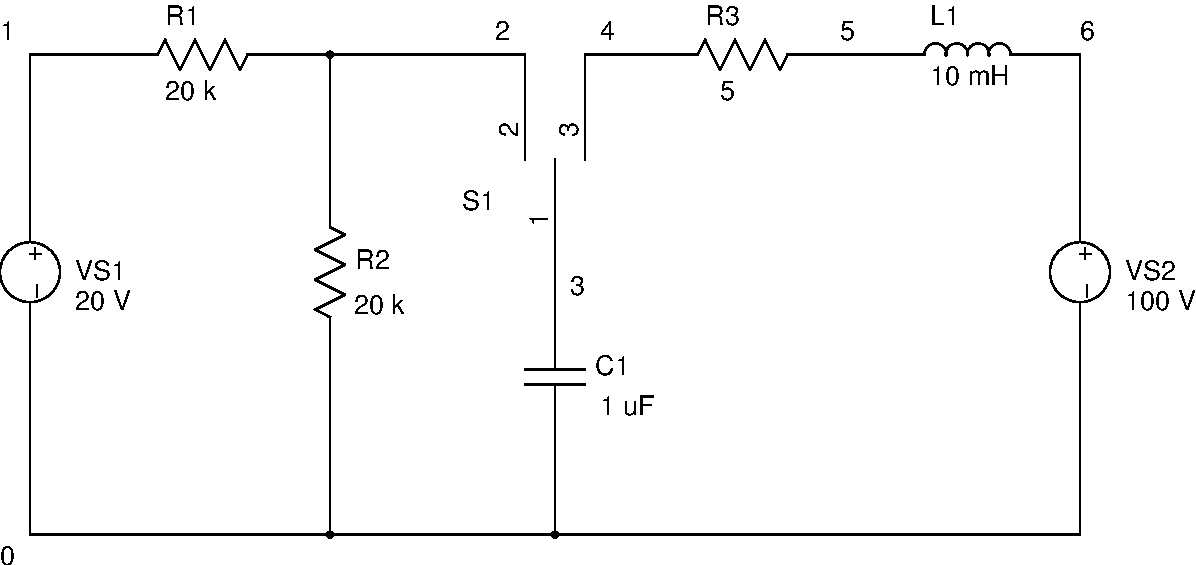
\includegraphics[scale=0.5]{spice/circuit-01}
\caption{Circuit definition.
Nodes denoted by numbers with 0 as common.
The switch (S1) starts at $t=0^-$ connected from terminals 1 to 2.
At $t=0$ it disconnects from 1 to 2 and connects to 1 to 3.
}
\label{fig:circuit}
\end{figure}

Unfortunately, due to the limitations of SPICE, the circuit can not be
implemented directly and must be modified.
The first difficulty is that there is no single pole double throw (SPDT) switch.
An equivalent can be accomplished using two single pole single throw (SPST)
switches.
The second problem is that switches cannot be triggered by time, they
can only be triggered by voltage changes.
The effect of triggering over time be accomplished using a pulsing voltage.
In order to read this pulsing voltage without disrupting the circuit being
analyzed an additional circuit will be added.
The modified version of this circuit is shown in Figure \ref{fig:circuit-02}.

\begin{figure}
\center
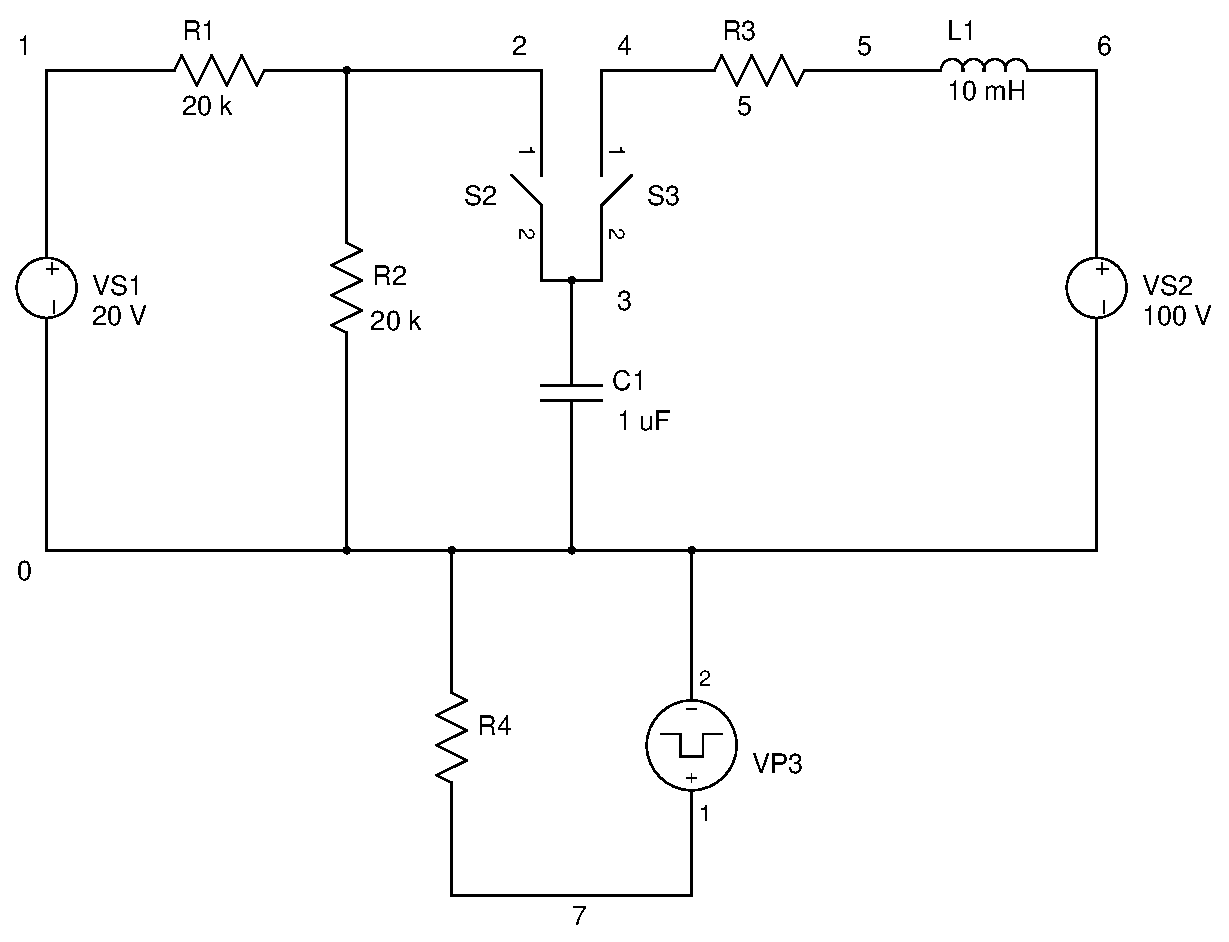
\includegraphics[scale=0.5]{spice/circuit-02}
\caption{Modification of original circuit definition (Figure \ref{fig:circuit})
to overcome the limitations of SPICE.
S2 and S3 are voltage controlled SPST switches that switch simultaneously.
At $t=0^-$ S2 is closed and S3 is open.  At $t=0$ S2 opens and S3 closes.
VP3 is a pulsing voltage source used to trigger the switches S2 and S3.
R4 is some resistor of arbitrary valued used to establish a measurable
voltage from VP3.
}
\label{fig:circuit-02}
\end{figure}

The SPICE definition is shown in Figure \ref{fig:spice}.

In general a SPICE simulation can be run using Ngspice with the command
\begin{verbatim}
  ngspice -b your_file.cir
\end{verbatim}
where \verb+your_file.cir+ replaced by the name of your file
containing the SPICE definition.
To save the output to a file a redirect can be used as in:
\begin{verbatim}
  ngspice -b your_file.cir > your_file.out
\end{verbatim}

\begin{figure}
\footnotesize
\verbatiminput{spice/circuit-02.cir}
\caption{SPICE definition of modified circuit definition (Figure \ref{fig:circuit-02}).}
\label{fig:spice}
\end{figure}

\clearpage
% }}}

% {{{ Results
\section{Results}

To assist in the analysis the time period was adjusted so
that a steady state was reached before the circuit was situated.
This also made it match the initial conditions.
Figure \ref{fig:capv} shows the voltage across the capacitor
during two periods.
It can be seen that there are two components: the under-damped RLC component
which oscillates rapidly and the RC component which gradually changes
without oscillation.

\begin{figure}
\center
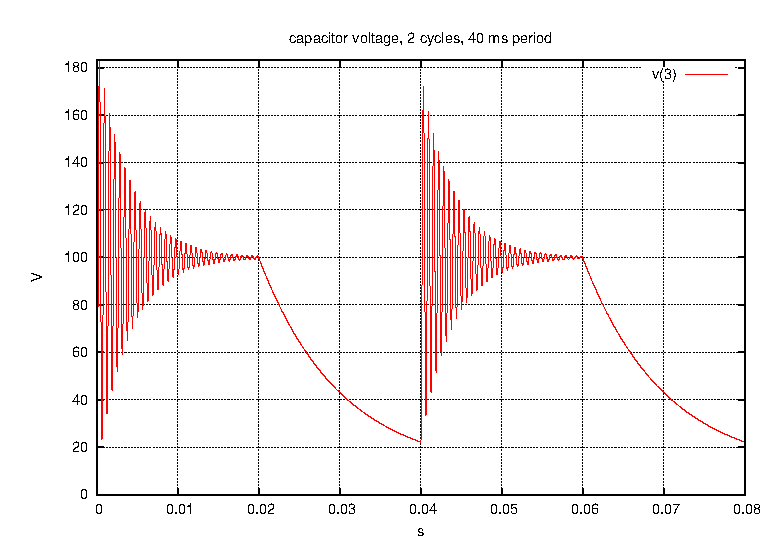
\includegraphics[scale=1.0]{spice/p_v3-80ms} \\
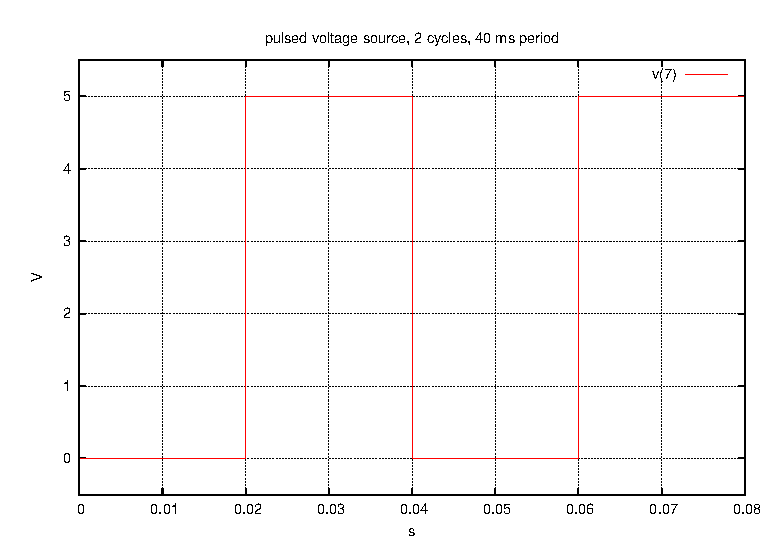
\includegraphics[scale=1.0]{spice/p_v7-80ms}
\caption{Capacitor voltage and pulsed voltage which controls the switch
over the same time period.
Two periods are shown (1 period equals 40 ms) and steady state conditions
are reached at each point (0, 40 ms, 80 ms).
}
\label{fig:capv}
\end{figure}

\clearpage

% }}}

% {{{ Correlation with theory
\section{Correlation with theory}

To assist conceptually, the two states of the modified circuit
(Figure \ref{fig:circuit-02}) are shown in Figure \ref{fig:circuit-03}.

\begin{figure}
\center
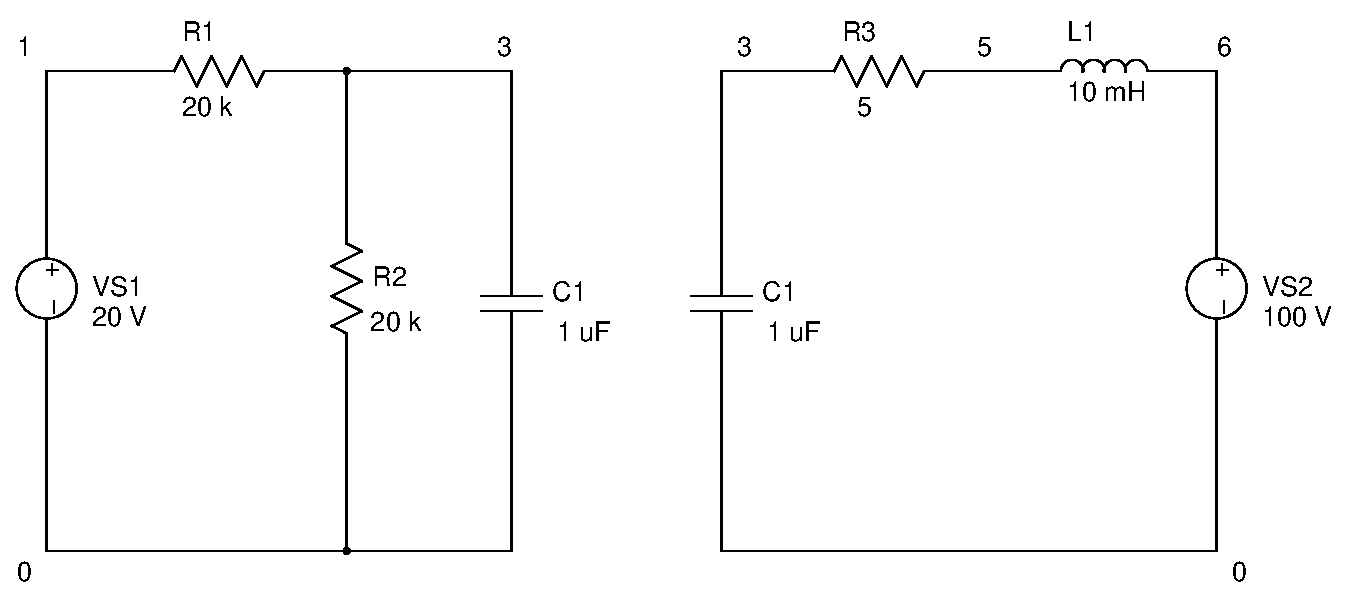
\includegraphics[scale=0.5]{spice/circuit-03}
\caption{The two states of the modified circuit (Figure \ref{fig:circuit-02}).
When the switch is connected to the left hand side the left most circuit
is active and similarly for the right hand side.
}
\label{fig:circuit-03}
\end{figure}

Starting with the left hand side (Figure \ref{fig:circuit-03}) this
circuit is equivalent to a RC circuit with a forced voltage.
Construction the equation for the step response of an RC circuit
results in Equation \ref{eq:rcstep}.
Substitution a time period of 20 ms results in a value of 22.1 volts
which is nearly the same as the value in Figure \ref{fig:capv}.

\begin{align}
	\frac{dv_C}{dt} + \frac{v_C}{R C} &= \frac{I_s}{C} \notag \\
	v_c &= I_s R + (V_0 - I_s R) e^{-t / RC} \notag \\
	v_c(t) &= (1 mA) (10k) + (100 - (1 mA) (10k)) e^{-t / (10k) (1 uF)} \notag \\
	v_c(t) &= 10 + 90 e^{-100 t} \label{eq:rcstep}
\end{align}


The right hand side of (Figure \ref{fig:circuit-03}) behaves like a
under-damped series RLC circuit with a forced component as can be seen by the rapid
oscillations in Figure \ref{fig:capv}.
Solving the equations results in the following:

\begin{align*}
	\alpha &= \frac{R}{2L} \\
			&= 250 \\
	\omega_0 &= \frac{1}{\sqrt{L C}} \\
			&= 10000 \\
	\alpha &< \omega_0 \quad\quad\quad \mbox{(under-damped)} \\
	\omega_d &= \sqrt{\omega_0^2 - \alpha^2} \\
		&= 10.0\e3 \quad \mbox{[rad/s]}
\end{align*}

\begin{align*}
	v_c(0^+) &= 22.1 \\
	v_f(\infty) &= 100 \\
	\frac{dv_c(0^+)}{dt} &= 0 \\
	v(0) &= v_f + \beta_1 \\
	\beta_1 &= 22.1 - 100 \\
			&= -77.9 \\
	0 &= - \alpha \beta_1 + \omega_d \beta_2 \\
	  &= 1.95\e4 + (10\e3) \beta_2 \\
	\beta_2 &= 1.94
\end{align*}

\begin{align}
	v(t) &= 100 + e^{-250 t} \left[ -77.9 \cos(10\e3 t) + 1.94 \sin(10\e3 t) \right] \label{eq:rlc}
\end{align}

And substituting values in to Equation \ref{eq:rlc} shows that it behaves
approximately according to figure \ref{fig:capv}.

\begin{align*}
\end{align*}

\clearpage

% }}}

% {{{ Conclusion
\section{Conclusion}

This experiment was a success in analyzing the behavior of first order
RC and RL circuits and second order RLC circuits under transient conditions
using a SPICE simulator.
The calculated values approximately matched the plotted values from
the SPICE output and agreed with the theory.

% }}}

% {{{ References
%\clearpage

%\pagebreak
\renewcommand*{\refname}{\vspace{-8mm}}
\section{References}
\bibliographystyle{ieeetr}
\bibliography{../references}
% }}}

\end{document}

% vim:foldmethod=marker

